\documentclass[12pt,a4paper]{article}
\usepackage[utf8]{inputenc}
\usepackage[T1]{fontenc}
%\usepackage[catalan]{babel}
\usepackage{amsmath, amssymb, amsfonts}
\usepackage{graphicx}
\usepackage{url}
\usepackage{comment}
\usepackage{booktabs}
\usepackage{array}
\usepackage[shortlabels]{enumitem}
\usepackage{xcolor}
\usepackage{pgfplots}
\usepackage{tcolorbox}
\usepackage{pdflscape}
\usepackage{makecell}
\usepackage{fancyhdr}
\usepackage[hidelinks]{hyperref}
\usepackage{tocloft}
\usepackage{geometry}
\usepackage{float}
\usepackage{tikz}
\usepackage{listings}
\usepackage{pdfpages}
\usetikzlibrary{trees}
\usetikzlibrary{shapes,arrows,positioning}

\geometry{a4paper, top=2.3cm, bottom=2cm, left=2.3cm, right=2.3cm}

\lstdefinestyle{mystyle}{
    backgroundcolor=\color{backcolour},   
    commentstyle=\color{codegreen},
    keywordstyle=\color{blue},
    numberstyle=\tiny\color{codegray},
    stringstyle=\color{codepurple},
    basicstyle=\ttfamily\small,
    breakatwhitespace=false,         
    breaklines=true,                 
    captionpos=b,                    
    keepspaces=true,                 
    numbers=left,                    
    numbersep=5pt,                  
    showspaces=false,                
    showstringspaces=false,
    showtabs=false,                  
    tabsize=2
}

\definecolor{codegreen}{rgb}{0,0.6,0}
\definecolor{codegray}{rgb}{0.5,0.5,0.5}
\definecolor{codepurple}{rgb}{0.58,0,0.82}
\definecolor{backcolour}{rgb}{0.95,0.95,0.92}

\lstset{style=mystyle}
\lstset{
  literate={á}{{\'a}}1 {é}{{\'e}}1 {í}{{\'i}}1 {ó}{{\'o}}1 {ú}{{\'u}}1
           {ü}{{\"u}}1 {ñ}{{\~n}}1 {ç}{{\c{c}}}1
}

% Define bag style for tikz
\tikzset{bag/.style={rectangle, draw}}

\title{\LARGE What is GraphQL}
\author{Aprenentatge i raonament automàtic}
\date{\today}

\pagestyle{fancy}
\fancyhf{}
\fancyhead[L]{GraphQL}
\fancyhead[R]{Distributed computing}

\fancyfoot[C]{\thepage}
\renewcommand{\headrulewidth}{0.4pt}
\renewcommand{\footrulewidth}{0.4pt}

\begin{document}

\begin{titlepage}
  \begin{center}

    \includegraphics[width=5cm]{udl.png}
    \hspace{0.2cm}
    \includegraphics[width=6cm]{eps.jpg}
    
    \vspace{1cm}
    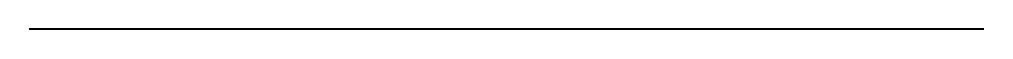
\begin{tikzpicture}[line width=1pt]
      \draw (0,0) -- (\textwidth,0);
    \end{tikzpicture}
    
    \vspace{3cm}
    {\LARGE \textbf{What's GraphQL}}

    \vspace{3cm}
    {\Large Activity 2: Distributed computing applications report}
    
    \vspace{3cm}
    
    \vfill
    {\Large \today}
    \vfill
    
    \vfill

    {\Large May Castells Raga \par}
    {\Large Anna Marin Nuño \par}
    \vfill
    
    \vspace{1cm}
    {\large Distributed Computing\\}
    {\large Grau en Enginyeria Informàtica\\}
    {\large Universitat de Lleida}
    
    \vspace{1cm}
    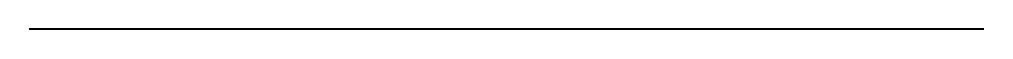
\begin{tikzpicture}[line width=1pt]
      \draw (0,0) -- (\textwidth,0);
    \end{tikzpicture}
  \end{center}
\end{titlepage}
\newpage

% Índice
%\renewcommand{\contentsname}{Índex}
\tableofcontents
\newpage

\section{Brief introduction}


In this project, we created a simple web service that uses four APIs to get information about animals and maps. The web service backend is built with FastAPI and the frontend with React. We started with a github simple template for FastAPI and React applications that the teacher showed us in class and then we added the required features and modified some behaviors to fit our needs.

% --- Landscape image page ---
\newpage
\begin{landscape}
\begin{figure}[H]
  \centering
  \includegraphics[width=0.95\linewidth]{architecture.drawio.png}
  \label{fig:project_overview}
  \caption{Project Overview}
\end{figure}
\end{landscape}
\newpage

\section{Login system}

The login system supports classic username/password (OAuth2) authentication with tokens as we did in class

\textbf{Frontend}: The login page collects user credentials and dispatches a Redux action (\texttt{login}). This calls an API function (\texttt{loginWithOauth}) that sends a POST request to \texttt{/login/oauth} with the username and password. If successful, the backend returns an \texttt{access\_token} and \texttt{refresh\_token}, which are stored in Redux state (\texttt{tokensSlice}).
  \textbf{Backend}: The \texttt{/login/oauth} endpoint (in \texttt{api/api\_v1/endpoints/login.py}) authenticates the user using the provided credentials. If valid, it generates an access token (short-lived JWT) and a refresh token (long-lived JWT, also stored in the DB for revocation). The access token is used for authenticating API requests.


\section{The distl: ETL Providers for Animal Data}

The ``distl'' (Data Integration Service Layer) is the part of the backend responsible for gathering, normalizing, and storing animal observation data from multiple external sources. We used 4 different APIs: eBird for bird observations, Wildlife for image-based animal recognition, Ninjas for general animal data, and OpenStreetMaps and Photon for geospatial data, basicaly for geocoding and getting coordinates.

The distl is a set of ETL (Extract, Transform, Load) providers. Each provider is a Python class that knows how to fetch data from a specific source (like eBird, Wildlife, or OpenStreetMaps), clean it up, and save it in our database in a consistent format. For example, the EBirdProvider connects to the eBird API, downloads recent bird observations, and transforms them into our internal schema. The same pattern is followed for other sources, each with its own provider class.

The ETL process works like this: first, the provider fetches raw data from the external API. Then, it normalizes the data, this means converting all the different field names, types, and structures into a common format that is used. Finally, the provider saves both the raw and normalized data in MongoDB, so can always trace back where each observation came from.

Since all ETL looked pretty similar, we created a base abstract class called \texttt{ETLProvider} that defines the common interface and shared functionality for all providers. Each specific provider (like \texttt{EBirdProvider}, \texttt{WildlifeProvider}, etc.) extends this base class and implements the details for its own data source. This design pattern is shown in the following diagram:

\begin{figure}[H]
    \centering
    \includegraphics[width=0.8\textwidth]{uml_dstl.drawio.png}
    \caption{ETL Providers Design Pattern}
    \label{fig:etl_providers}
\end{figure}


\subsection{EBirdProvider}

The \texttt{EBirdProvider} extends \texttt{ETLProvider} and is responsible for importing bird data from the eBird API. It sets up API keys, URLs, and a logger in its constructor. The method \texttt{get\_species\_codes} looks up eBird species codes for a given common name, using a cached taxonomy. The \texttt{fetch} method downloads raw bird observation data, handling retries and deduplication. The \texttt{normalize} method converts eBird data into the internal schema, mapping fields like species, sci\_name, lat, lon, date, location, how\_many, and obs\_id. There are also methods to save raw and normalized data (\texttt{save\_raw\_data}, \texttt{save\_normalized\_data}), and \texttt{get\_observations} retrieves recent observations for a species from the database, using cache if available.

\subsection{WildlifeProvider}

The \texttt{WildlifeProvider} is for the Wildlife API. It sets up API keys and URLs in its constructor. The \texttt{fetch} method handles image preprocessing (resizing or compressing if needed)\footnote{Compressing is a key part because Wildlife API imagee limit size is 5MB and the total API usage is 1GB}, sends the image to the Wildlife API, and returns the response. The \texttt{normalize} method extracts and standardizes annotation data (id, label, confidence, taxonomy, bbox) from the API response.

\subsection{NinjasProvider}

The \texttt{NinjasProvider} is for the Ninjas API. It sets up API keys and URLs in its constructor. The \texttt{fetch} method queries the Ninjas API for animal data by name, tries fallback strategies if no results, and filters results. The \texttt{normalize} method converts the Ninjas API response into a list of dictionaries with name, taxonomy, locations, and characteristics. The \texttt{save} method saves both raw and normalized data to the database.

\subsection{OpenStreetMapsProvider}

The \texttt{OpenStreetMapsProvider} is for geospatial data and geocoding. It sets up API keys and Photon geocoding service URLs in its constructor. The provider has several methods: \texttt{get\_map\_for\_locations} takes a list of locations, queries Photon (an OpenStreetMap geocoder) for each one, extracts coordinates, and returns them along with a computed center point. The \texttt{fetch} method queries the Photon API for geocoding results given a location query string. The \texttt{normalize} method converts Photon/OSM data into a list of dictionaries with place\_id, name, coordinates, type, and class. Additionally, \texttt{geocode\_single} takes a single location string and returns a tuple of latitude and longitude coordinates, while \texttt{reverse\_geocode\_country} takes latitude and longitude coordinates and returns the country code by performing reverse geocoding.

All providers follow the same pattern: fetch data from their source, normalize it, and store it in MongoDB. Each provider handles the requirements of its own API, so the rest of the application can work with a unified data model.

\section{API Endpoints Documentation}

The backend exposes several REST API endpoints organized into three main categories: user management, analytical endpoints, and ETL system management. All endpoints require authentication via JWT access tokens (except login/register).

\subsection{User Management Endpoints}

\subsubsection{POST /api/v1/login/oauth}
Authenticates a user with username and password using OAuth2 standard. Receives form data with \texttt{username} and \texttt{password} fields. Returns an access token (JWT, 30-minute expiry) and a refresh token (JWT, 30-day expiry). The refresh token is stored in the database for revocation control. Possible responses: 200 with token payload, 400 for incorrect credentials, or 401 for inactive users.

\subsubsection{POST /api/v1/login/refresh}
Refreshes an expired access token using a valid refresh token. Receives the refresh token in the request body. Validates the token signature and checks if it exists in the database (not revoked). Returns a new access token. Possible responses: 200 with new token, 401 if token is invalid or revoked, 404 if token not found in database.

\subsubsection{POST /api/v1/login/logout}
Revokes the current user's refresh token, effectively logging them out. Requires authentication via access token. Removes the refresh token from the database. Returns a success message. Possible responses: 200 with confirmation message, 401 if not authenticated.

\subsubsection{GET /api/v1/users/}
Retrieves the current authenticated user's profile information. Requires valid access token. Returns user data including id, email, username, full name, role, and active status. Possible responses: 200 with user object, 401 if not authenticated.

\subsubsection{GET /api/v1/users/all}
Lists all users in the system (admin only). Requires admin role. Supports pagination with \texttt{skip} and \texttt{limit} query parameters. Returns array of user objects. Possible responses: 200 with user list, 401 if not authenticated, 403 if not admin.

\subsubsection{POST /api/v1/users/create}
Creates a new user account (admin only). Receives user data in request body: email, username, password, full name, and optional role. Validates email uniqueness and password strength. Returns the created user object. Possible responses: 201 with new user, 400 if email already exists, 401 if not authenticated, 403 if not admin.

\subsubsection{PUT /api/v1/users/\{user\_id\}}
Updates an existing user's information. Users can update their own profile; admins can update any user. Receives partial user data to update. Returns the updated user object. Possible responses: 200 with updated user, 401 if not authenticated, 403 if insufficient permissions, 404 if user not found.

\subsubsection{DELETE /api/v1/users/\{user\_id\}}
Deletes a user account (admin only). Permanently removes the user from the database. Returns the deleted user object. Possible responses: 200 with deleted user, 401 if not authenticated, 403 if not admin, 404 if user not found.

\subsubsection{PUT /api/v1/users/\{user\_id\}/role}
Changes a user's role (admin only). Receives new role in request body (\texttt{user} or \texttt{admin}). Updates the user's role in the database. Returns the updated user object. Possible responses: 200 with updated user, 401 if not authenticated, 403 if not admin, 404 if user not found.

\subsection{Analytical Endpoints}

\subsubsection{POST /api/v1/image-upload/image-to-animal-info}
Identifies animals in an uploaded image using the Wildlife API. Receives a multipart form with an image file. Sends the image to WildlifeProvider which processes it (resizes/compresses if needed), queries the Wildlife API, and returns identified species with confidence scores, bounding boxes, and taxonomy information. Called from the frontend's image-to-animal page. Possible responses: 200 with array of detected animals, 400 if no file provided, 401 if not authenticated, 500 if Wildlife API fails.

\subsubsection{GET /api/v1/maps/geocode}
Converts location names to geographic coordinates using Photon/OpenStreetMap geocoding. Receives a \texttt{query} parameter with the location string. Uses OpenStreetMapsProvider to query Photon API and returns latitude, longitude, and place metadata. Called from frontend map components. Possible responses: 200 with geocoding results, 400 if query is empty, 401 if not authenticated, 404 if location not found.

\subsubsection{POST /api/v1/maps/animal-to-map}
Creates a map visualization showing locations where specific animals have been observed. Receives an array of location names in the request body. For each location, geocodes it using OpenStreetMapsProvider (returns only the first/best coordinate match per location to avoid duplicates), retrieves eBird observations for that area, and returns coordinates plus a computed center point for map rendering. Called from the frontend's animal-to-map page. Possible responses: 200 with location coordinates and center, 401 if not authenticated, 500 if geocoding fails.

\subsubsection{GET /api/v1/maps/ebird-observations-map}
Retrieves eBird bird observations for map display. Receives optional query parameters for filtering: \texttt{species\_code}, \texttt{region\_code}, \texttt{back} (days back), and \texttt{max\_results}. Uses EBirdProvider to fetch observations from eBird API, normalizes the data, and returns observation points with coordinates. Called from frontend map visualization components. Possible responses: 200 with observation array, 401 if not authenticated, 500 if eBird API fails.

\subsubsection{GET /api/v1/observations/search}
Searches for animal observations across multiple data sources. Receives optional query parameters: \texttt{species\_name}, \texttt{common\_name}, \texttt{location}, \texttt{start\_date}, \texttt{end\_date}, \texttt{source} (ebird, wildlife, ninjas). Queries MongoDB observations collection with filters, performs text search if species name provided, and returns matching observations with pagination. Called from frontend search interfaces. Possible responses: 200 with search results and total count, 401 if not authenticated.

\subsection{ETL System Endpoints}

\subsubsection{POST /api/v1/disl/\{provider\}/run}
Triggers an ETL process for a specific data provider. Receives \texttt{provider} path parameter (ebird, wildlife, ninjas, or openstreetmaps) and optional query parameters specific to each provider (e.g., species name for eBird, location for maps). Instantiates the corresponding ETLProvider class, executes the fetch-normalize-save pipeline, and returns the processed results. Can run as background task for long operations. Called from frontend data ingestion interfaces or admin panels. Possible responses: 200 with ETL results, 400 if invalid provider or parameters, 401 if not authenticated, 500 if ETL process fails.

\subsubsection{GET /api/v1/disl/\{provider\}/results}
Retrieves the most recent results from a specific ETL provider. Receives \texttt{provider} path parameter. Queries the raw\_data or observations collection for the latest entries from that provider. Returns normalized data that was previously extracted. Useful for checking what data was last imported. Possible responses: 200 with result array, 401 if not authenticated, 404 if no results found.

\subsubsection{GET /api/v1/disl/\{provider\}/history}
Fetches historical ETL execution logs for a provider. Receives \texttt{provider} path parameter and optional pagination parameters. Returns metadata about past ETL runs including timestamps, record counts, success/failure status, and error messages. Useful for monitoring and debugging data pipelines. Possible responses: 200 with execution history, 401 if not authenticated.

\subsubsection{GET /api/v1/analytics/temporal-patterns}
Analyzes temporal patterns in animal observations. Receives optional query parameters: \texttt{species}, \texttt{location}, \texttt{time\_granularity} (hour, day, month, year). Aggregates observation data by time periods, calculates frequencies, identifies peak activity times, and returns statistical summaries. Uses MongoDB aggregation pipeline for efficient time-series analysis. Called from frontend analytics dashboards. Possible responses: 200 with temporal analysis results, 401 if not authenticated, 400 if invalid parameters.


\section{User and admin interface}

The interface of our application is quite simple since we wanted to spend more time and resources on the backend. It consists of a public section open to all users containing a page for each function of the app and an admin page exclusive to admin users where they can moderate users and keep an eye on the logs.

\subsection{Public section}

\subsubsection{Image to animal}

\begin{figure}[htp]
    \centering
    \includegraphics[width=8cm]{image-to-animal.png}
    \caption{An example of the page Image to animal}
    \label{fig:Image to animal example}
\end{figure}

Image to Animal lets the user upload an image of an animal and have it identified by Wildlife API and Ninjas API. Once the animal is identified, the user has the option to see where that animal has been seen recently, an action that will bring them to the next page.

\subsubsection{Locate animal on map}

\begin{figure}[htp]
    \centering
    \includegraphics[width=8cm]{locate-to-map.png}
    \caption{An example of the page Locate animal on map}
    \label{fig:Locate animal on map example}
\end{figure}

In Locate animal on Map, the user can introduce an animal to search the recent location of the specific animal using the Ninja API and displaying the results on a world map.

\subsubsection{Bird observation}
\begin{figure}[htp]
    \centering
    \includegraphics[width=8cm]{bird-observations.png}
    \caption{An example of the page bird observations}
    \label{fig: bird observations example}
\end{figure}

Bird observations uses the eBird API to search for the recent observations of different species of birds and then displays them in a world map.

\subsubsection{Map search}

\begin{figure}[htp]
    \centering
    \includegraphics[width=8cm]{observations.png}
    \caption{An example of the page Map search}
    \label{fig: bird map search example}
\end{figure}

In Map Search, users can search for a specific country to see the different species spotted in that country provided by the eBird API and our database.


\subsubsection{Temporal activity patterns}

\begin{figure}[htp]
    \centering
    \includegraphics[width=8cm]{analysis.png}
    \caption{An example of the page Temporal activity patterns}
    \label{fig:Temporal activity patterns example}
\end{figure}


Temporal activity patterns combine the results of eBird and the Ninjas API, and it analyzes them to provide an activity graph for a specific species, including the best time to spot that animal and the environment they inhabit the most.

\section{Logging System}

The application implements a comprehensive logging system that tracks both user authentication activities and ETL (Extract, Transform, Load) operations. The logging infrastructure uses Python's built-in logging module and stores structured log data in MongoDB for persistent audit trails.

\subsection{Login Logging}

The login logging system tracks all authentication attempts in the application, storing them in a dedicated MongoDB collection for security auditing and monitoring purposes.

\subsubsection{Implementation}

Login logs are created automatically during the OAuth2 authentication process. When a user attempts to log in via the \texttt{POST /api/v1/login/oauth} endpoint, the system performs the following steps:

\begin{enumerate}
    \item The endpoint receives username (email) and password from the OAuth2 form data
    \item The system attempts to authenticate the user using \texttt{crud.user.authenticate()}
    \item A login log entry is created with a \texttt{LoginLogCreate} schema containing:
    \begin{itemize}
        \item \texttt{email}: The email/username used in the login attempt
        \item \texttt{success}: Boolean indicating whether the login was successful (user exists and is active)
        \item \texttt{timestamp}: Automatically added by the database (current UTC time)
    \end{itemize}
    \item The log entry is persisted to MongoDB via \texttt{crud.login\_log.create()}
    \item If authentication succeeds, access and refresh tokens are generated and returned
    \item If authentication fails, an HTTP 401 error is raised (after the log has been created)
\end{enumerate}

\subsubsection{Data Schema}

The \texttt{LoginLog} schema (defined in \texttt{app/schemas/}) contains the following fields:

\begin{itemize}
    \item \texttt{id}: MongoDB ObjectId converted to string
    \item \texttt{email}: User's email address used in login attempt
    \item \texttt{success}: Boolean indicating successful authentication and active user status
    \item \texttt{timestamp}: UTC datetime when the login attempt occurred
\end{itemize}

\subsubsection{Retrieval and Admin Access}

Login logs can be retrieved through the \texttt{GET /api/v1/login-logs/} endpoint, which is restricted to superuser/admin access only. The endpoint implements:

\begin{itemize}
    \item Pagination support via \texttt{skip} and \texttt{limit} query parameters
    \item Descending chronological ordering (most recent first)
    \item Backward compatibility handling for legacy log entries that may lack certain fields
    \item Automatic email resolution for older logs that stored \texttt{user\_id} instead of \texttt{email}
\end{itemize}

The retrieval process includes data normalization to handle database schema evolution:

\begin{lstlisting}[language=Python]
# Ensure all required fields exist with defaults
if "timestamp" not in doc:
    doc["timestamp"] = datetime.now()
if "success" not in doc:
    doc["success"] = True
# Handle legacy documents with user_id
if "email" not in doc and "user_id" in doc:
    user = await crud.user.get(db, id=doc["user_id"])
    doc["email"] = user.email if user else "unknown@example.com"
\end{lstlisting}

\subsection{ETL Logging}

The ETL logging system provides detailed operational logs for all data extraction, transformation, and loading processes across multiple external APIs. Each ETL provider implements structured logging to track the complete data pipeline lifecycle.

\subsubsection{Base ETL Logging Infrastructure}

All ETL providers extend the abstract \texttt{ETLProvider} base class, which provides centralized logging utilities:

\begin{lstlisting}[language=Python]
def get_logger(self):
    return logging.getLogger(f"app.services.disl.{self.source.value}")

def log_info(self, message: str):
    self.get_logger().info(f"[{self.source.value}] {message}")

def log_warning(self, message: str):
    self.get_logger().warning(f"[{self.source.value}] {message}")

def log_error(self, message: str):
    self.get_logger().error(f"[{self.source.value}] {message}")
\end{lstlisting}

Each provider gets a named logger based on its data source (e.g., \texttt{app.services.disl.ebird}, \texttt{app.services.disl.wildlife}), ensuring log messages are properly categorized and can be filtered by source.

\subsubsection{EBird Provider Logging}

The \texttt{EBirdProvider} implements comprehensive logging throughout its ETL pipeline:

\begin{itemize}
    \item \textbf{ETL Start}: Logs when an ETL process begins, including region code and species query\\
    \texttt{[EBIRD-ETL] Starting ETL for region: US, species query: eagle}
    
    \item \textbf{Data Fetch}: Logs the number of records fetched from eBird API\\
    \texttt{[EBIRD-ETL] Fetched 150 records from eBird for US}
    
    \item \textbf{Normalization}: Logs the number of records normalized into internal schema\\
    \texttt{[EBIRD-ETL] Normalized 150 records.}
    
    \item \textbf{ETL Complete}: Logs successful completion with final record count\\
    \texttt{[EBIRD-ETL] ETL complete. Saved 150 records.}
    
    \item \textbf{Cache Events}: Logs when cached data is used instead of triggering new ETL\\
    \texttt{[EBIRD-PROVIDER] No cached observations for eagle, triggering ETL.}
\end{itemize}

\subsubsection{Maps Provider Logging}

The \texttt{OpenStreetMapsProvider} logs all geocoding operations with detailed context:

\begin{itemize}
    \item \textbf{Process Start}: Logs the beginning of geocoding for a set of locations\\
    \texttt{[ETL-MAP] Starting get\_map\_for\_locations for: ['Africa', 'Asia']}
    
    \item \textbf{Individual Queries}: Logs each Photon API query\\
    \texttt{[ETL-MAP] Querying Photon for: Africa}
    
    \item \textbf{Results}: Logs the number of coordinates found per location\\
    \texttt{[ETL-MAP] Found 5 coordinates for Africa, using the first one}
    
    \item \textbf{Warnings}: Logs when no coordinates are found\\
    \texttt{[ETL-MAP] No coordinates found for location: InvalidPlace}
    
    \item \textbf{Errors}: Logs failures with error details and timeout detection\\
    \texttt{[ETL-MAP] Timeout fetching coordinates from Photon for Europe - location may be too broad or API is slow}
    
    \item \textbf{Process Complete}: Logs total coordinates retrieved\\
    \texttt{[ETL-MAP] Finished. Total coordinates: 10}
    
    \item \textbf{Reverse Geocoding}: Logs successful country code resolution\\
    \texttt{Reverse geocoded (41.5, 2.1) to country: ES}
\end{itemize}

\subsubsection{Wildlife Provider Logging}

The \texttt{WildlifeProvider} logs image processing and API interactions:

\begin{itemize}
    \item \textbf{API Responses}: Logs raw Wildlife API responses for debugging\\
    \texttt{Wildlife API response: \{"annotations": [...]\}}
    
    \item \textbf{Image Processing}: Logs when images are resized or compressed (in \texttt{image\_utils.py})\\
    \texttt{Image resized/compressed to 2048576 bytes, quality=85}
\end{itemize}

\subsubsection{Ninjas Provider Logging}

The \texttt{NinjasProvider} logs API queries and fallback strategies:

\begin{itemize}
    \item \textbf{Primary Query}: Logs API responses for initial queries\\
    \texttt{Ninjas API response for 'bald eagle': [...]}
    
    \item \textbf{Fallback Strategy}: Logs when using last-word fallback for multi-word species names\\
    \texttt{No results for 'bald eagle', trying last word: 'eagle'}\\
    \texttt{Ninjas API response for 'eagle': [...]}
\end{itemize}

\subsubsection{Error Tracking and Database Storage}

The base \texttt{ETLProvider} class includes a \texttt{store()} method that persists both successful and failed ETL operations to MongoDB:

\begin{lstlisting}[language=Python]
async def store(self, data: Any, status: ETLStatus, 
                error: Optional[str] = None, 
                metadata: Optional[dict] = None):
    raw_data_doc = {
        "source": self.source.value,
        "data": data,
        "fetched_at": datetime.utcnow(),
        "status": status.value,
        "error_message": error,
        "metadata": metadata or {}
    }
    await self.db["raw_data"].insert_one(raw_data_doc)
    logger.info(f"Stored data for {self.source} with status {status}")
\end{lstlisting}

This creates a permanent audit trail of all ETL executions, including:
\begin{itemize}
    \item Data source identifier
    \item Fetched data (or null on failure)
    \item Timestamp of execution
    \item Success/failure status
    \item Error messages for failed operations
    \item Custom metadata (e.g., query parameters, record counts)
\end{itemize}

\subsubsection{Log Output and Monitoring}

All logs are written to standard output in the Docker container environment, making them visible via \texttt{docker compose logs backend}. The structured format with source prefixes (e.g., \texttt{[EBIRD-ETL]}, \texttt{[ETL-MAP]}) enables easy filtering and monitoring of specific data pipelines. Log levels (INFO, WARNING, ERROR) allow operators to quickly identify issues requiring attention.

\end{document}



